\appendix
\chapter{BERTScore analysis}\label{chap:bertscore_analysis}
To evaluate the effectiveness of BERTScore in accurately assessing message quality, I analyzed the responses produced by the model alongside random commit messages. As a dataset for this experiment I used the CommitChronicle validation set. As a model to generate the messages, I used the base version of CodeT5+ to generate the messages. As a base BERT model for the BERTScore, i used the default BERT base uncased to enhance the calculation speed.
The results of the comparison are presented in Fig.~\ref{fig:BERTSCORE_analysis}. Y axis of this plot shows the BERTScore of a certain sample, and the x axis represents the length of code changes in this sample in characters. As is visible from the plot, the results of the generated messages strongly outperform the irrelevant random commit messages from the dataset. Therefore, I can conclude that the metric correctly measures the quality of the generated commit messages even with the base model.

\begin{figure}[H]
    % \hspace*{-1.5cm}
    \centering
    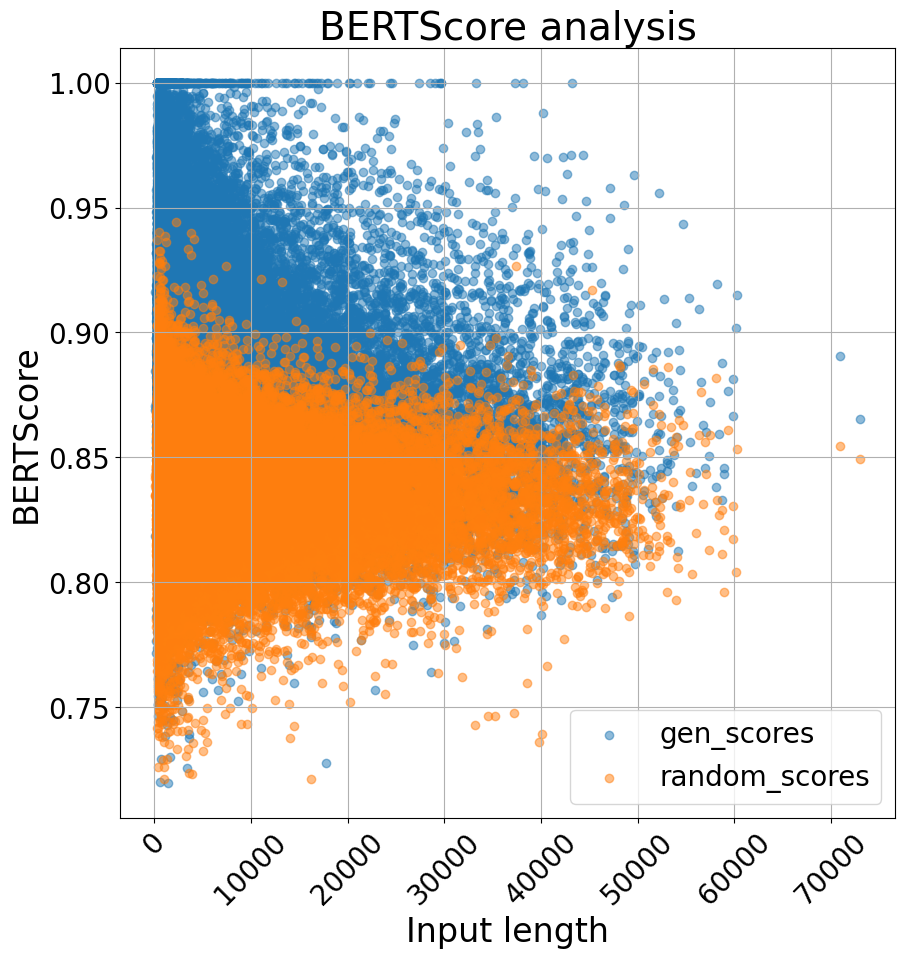
\includegraphics[scale=0.7]{figs/BERTScore analysis.png}
    \caption{Comparing the BERTScore of generated messages and random ones.}
    ~\label{fig:BERTSCORE_analysis}
\end{figure}

\chapter{Inference examples}
In this section, I present the inference results of my models. 
As an example for the inference, I used the random commit from the official PyTorch repository. The source of this commit can be found in the following \href{https://github.com/pytorch/pytorch/commit/3f11958d390feefcc0f4b629b089bfa6acc9c021}{GitHub link}. This commit changes the changes the content of some Dockefiles and shell scripts in the repository. It covers six different files and makes seven insertions and nine deletions. The inference results for all models and the true commit message for this commit are presented in Table~\ref{tab:inference}. The source code for this commit is presented below.
\setcounter{table}{14}
\begin{table}[h]
    \centering
    \caption{Inference results}\label{tab:inference}
    \renewcommand{\arraystretch}{1.5} % Adjusts the row height
    \begin{tabular}{| l | p{6cm} |} % chktex 44
    \hline % chktex 44
    \textbf{Model} & \textbf{Message} \\
    \hline % chktex 44
    CodeT5+ 220M & "[CI] Install libopencv-dev and ffmpeg-devel in Ubuntu Dockerfiles" \\ 
    \hline
    CodeT5+ 770M & "[CI] Remove ffmpeg and libavcodec from docker images" \\ 
    \hline
    CodeT5+ with file attention & "ci: remove ffmpeg from docker image" \\
    \hline 
    \multirow{2}{*}{\begin{tabular}[c]{@{}l@{}}CodeT5+ with file attention \\ single commit train\end{tabular}} & \multirow{2}{=}{\raggedright "ci: install ffmpeg and libopencv"} \\ 
    & \\
    \hline
    CodeT5+ with retrieval & "Remove ffmpeg from vision docker images"\\
    \hline
    \hline
    JetBrains CodeT5 & "Remove ffmpeg from Dockerfiles" \\ 
    \hline
    \textbf{Original message} & Remove FFMPEG from CI scripts (\#125546) Because FFMPEG was solely used by Caffe2. \\ 
    \hline
    \end{tabular}
\end{table}


\includepdf[pages={1-4}, offset=3cm -2cm]{chapters/untitled.pdf}